% Options for packages loaded elsewhere
\PassOptionsToPackage{unicode}{hyperref}
\PassOptionsToPackage{hyphens}{url}
\PassOptionsToPackage{dvipsnames,svgnames,x11names}{xcolor}
%
\documentclass[
  letterpaper,
  DIV=11,
  numbers=noendperiod]{scrartcl}

\usepackage{amsmath,amssymb}
\usepackage{iftex}
\ifPDFTeX
  \usepackage[T1]{fontenc}
  \usepackage[utf8]{inputenc}
  \usepackage{textcomp} % provide euro and other symbols
\else % if luatex or xetex
  \usepackage{unicode-math}
  \defaultfontfeatures{Scale=MatchLowercase}
  \defaultfontfeatures[\rmfamily]{Ligatures=TeX,Scale=1}
\fi
\usepackage{lmodern}
\ifPDFTeX\else  
    % xetex/luatex font selection
\fi
% Use upquote if available, for straight quotes in verbatim environments
\IfFileExists{upquote.sty}{\usepackage{upquote}}{}
\IfFileExists{microtype.sty}{% use microtype if available
  \usepackage[]{microtype}
  \UseMicrotypeSet[protrusion]{basicmath} % disable protrusion for tt fonts
}{}
\makeatletter
\@ifundefined{KOMAClassName}{% if non-KOMA class
  \IfFileExists{parskip.sty}{%
    \usepackage{parskip}
  }{% else
    \setlength{\parindent}{0pt}
    \setlength{\parskip}{6pt plus 2pt minus 1pt}}
}{% if KOMA class
  \KOMAoptions{parskip=half}}
\makeatother
\usepackage{xcolor}
\setlength{\emergencystretch}{3em} % prevent overfull lines
\setcounter{secnumdepth}{5}
% Make \paragraph and \subparagraph free-standing
\ifx\paragraph\undefined\else
  \let\oldparagraph\paragraph
  \renewcommand{\paragraph}[1]{\oldparagraph{#1}\mbox{}}
\fi
\ifx\subparagraph\undefined\else
  \let\oldsubparagraph\subparagraph
  \renewcommand{\subparagraph}[1]{\oldsubparagraph{#1}\mbox{}}
\fi


\providecommand{\tightlist}{%
  \setlength{\itemsep}{0pt}\setlength{\parskip}{0pt}}\usepackage{longtable,booktabs,array}
\usepackage{calc} % for calculating minipage widths
% Correct order of tables after \paragraph or \subparagraph
\usepackage{etoolbox}
\makeatletter
\patchcmd\longtable{\par}{\if@noskipsec\mbox{}\fi\par}{}{}
\makeatother
% Allow footnotes in longtable head/foot
\IfFileExists{footnotehyper.sty}{\usepackage{footnotehyper}}{\usepackage{footnote}}
\makesavenoteenv{longtable}
\usepackage{graphicx}
\makeatletter
\def\maxwidth{\ifdim\Gin@nat@width>\linewidth\linewidth\else\Gin@nat@width\fi}
\def\maxheight{\ifdim\Gin@nat@height>\textheight\textheight\else\Gin@nat@height\fi}
\makeatother
% Scale images if necessary, so that they will not overflow the page
% margins by default, and it is still possible to overwrite the defaults
% using explicit options in \includegraphics[width, height, ...]{}
\setkeys{Gin}{width=\maxwidth,height=\maxheight,keepaspectratio}
% Set default figure placement to htbp
\makeatletter
\def\fps@figure{htbp}
\makeatother
% definitions for citeproc citations
\NewDocumentCommand\citeproctext{}{}
\NewDocumentCommand\citeproc{mm}{%
  \begingroup\def\citeproctext{#2}\cite{#1}\endgroup}
\makeatletter
 % allow citations to break across lines
 \let\@cite@ofmt\@firstofone
 % avoid brackets around text for \cite:
 \def\@biblabel#1{}
 \def\@cite#1#2{{#1\if@tempswa , #2\fi}}
\makeatother
\newlength{\cslhangindent}
\setlength{\cslhangindent}{1.5em}
\newlength{\csllabelwidth}
\setlength{\csllabelwidth}{3em}
\newenvironment{CSLReferences}[2] % #1 hanging-indent, #2 entry-spacing
 {\begin{list}{}{%
  \setlength{\itemindent}{0pt}
  \setlength{\leftmargin}{0pt}
  \setlength{\parsep}{0pt}
  % turn on hanging indent if param 1 is 1
  \ifodd #1
   \setlength{\leftmargin}{\cslhangindent}
   \setlength{\itemindent}{-1\cslhangindent}
  \fi
  % set entry spacing
  \setlength{\itemsep}{#2\baselineskip}}}
 {\end{list}}
\usepackage{calc}
\newcommand{\CSLBlock}[1]{\hfill\break\parbox[t]{\linewidth}{\strut\ignorespaces#1\strut}}
\newcommand{\CSLLeftMargin}[1]{\parbox[t]{\csllabelwidth}{\strut#1\strut}}
\newcommand{\CSLRightInline}[1]{\parbox[t]{\linewidth - \csllabelwidth}{\strut#1\strut}}
\newcommand{\CSLIndent}[1]{\hspace{\cslhangindent}#1}

\KOMAoption{captions}{tableheading}
\makeatletter
\@ifpackageloaded{caption}{}{\usepackage{caption}}
\AtBeginDocument{%
\ifdefined\contentsname
  \renewcommand*\contentsname{Table of contents}
\else
  \newcommand\contentsname{Table of contents}
\fi
\ifdefined\listfigurename
  \renewcommand*\listfigurename{List of Figures}
\else
  \newcommand\listfigurename{List of Figures}
\fi
\ifdefined\listtablename
  \renewcommand*\listtablename{List of Tables}
\else
  \newcommand\listtablename{List of Tables}
\fi
\ifdefined\figurename
  \renewcommand*\figurename{Figure}
\else
  \newcommand\figurename{Figure}
\fi
\ifdefined\tablename
  \renewcommand*\tablename{Table}
\else
  \newcommand\tablename{Table}
\fi
}
\@ifpackageloaded{float}{}{\usepackage{float}}
\floatstyle{ruled}
\@ifundefined{c@chapter}{\newfloat{codelisting}{h}{lop}}{\newfloat{codelisting}{h}{lop}[chapter]}
\floatname{codelisting}{Listing}
\newcommand*\listoflistings{\listof{codelisting}{List of Listings}}
\makeatother
\makeatletter
\makeatother
\makeatletter
\@ifpackageloaded{caption}{}{\usepackage{caption}}
\@ifpackageloaded{subcaption}{}{\usepackage{subcaption}}
\makeatother
\ifLuaTeX
  \usepackage{selnolig}  % disable illegal ligatures
\fi
\usepackage{bookmark}

\IfFileExists{xurl.sty}{\usepackage{xurl}}{} % add URL line breaks if available
\urlstyle{same} % disable monospaced font for URLs
\hypersetup{
  pdftitle={Conditional Decompositions},
  pdfauthor={Michael Betancourt},
  colorlinks=true,
  linkcolor={blue},
  filecolor={Maroon},
  citecolor={Blue},
  urlcolor={Blue},
  pdfcreator={LaTeX via pandoc}}

\title{Conditional Decompositions}
\author{Michael Betancourt}
\date{August 2026}

\begin{document}
\maketitle
\begin{abstract}
All probability theory chapters can be found
\href{http://www.symplectomorphic.com/writing/\#part1}{here}.

A repository containing all of the files used to generate this chapter
is available on
\href{https://github.com/betanalpha/quarto_chapters/tree/main/10_probability_on_product_spaces}{GitHub}.
\end{abstract}

\renewcommand*\contentsname{Table of contents}
{
\hypersetup{linkcolor=}
\setcounter{tocdepth}{3}
\tableofcontents
}
\newcommand{\I}[2]{\mathbb{I}_{#1} \! \left[ #2 \right]}

\newcommand{\E}[2]{\mathbb{E}_{#1} \! \left[ #2 \right]}

\newcommand{\rnd}[2]{\frac{ \mathrm{d} #1}{ \mathrm{d} #2 }}

On
\href{http://www.symplectomorphic.com/assets/chapters_html/probability_theory_on_product_spaces}{product
spaces}, conditional probability theory becomes particularly useful when
we apply it more than once. After disintegrating a joint probability
distribution into a marginal distribution and conditional probability
kernel, we can often disintegrate that marginal distribution into even
simpler pieces.

In this chapter, we'll explore these recursive decompositions and their
organization into \emph{conditional decompositions}.

\section{Recursive Decomposition}\label{recursive-decomposition}

Recall that any subsequence of component indices, \[
\mathsf{i} \, \vec{\subset} \, 1:I,
\] defines a projection function \(\varpi_{ \mathsf{i} }\) that
disintegrates a joint probability distribution \[
\pi ( \mathsf{x}_{1:I} )
\] into a marginal distribution over the thinned product space
\(X^{\mathsf{i}}\), \[
\pi ( \mathsf{x}_{\mathsf{i}} ),
\] and a conditional probability kernel over the cross sections
\(X^{ \mathsf{i}^{c} } \times \{ x_{ \mathsf{i} }  )\), \[
\pi(
  \mathsf{x}_{\mathsf{i}^{c}} \mid
  x_{ \mathsf{i} }
).
\]

The marginal and conditional probability distributions will always be
simpler than the joint distribution, but they might not be simpler
enough for practical applications. Fortunately, the marginal
distribution is amenable to decomposition of its own.

A smaller subsequence of component indices, \[
\mathsf{i}' \, \vec{\subset} \,
\mathsf{i}  \, \vec{\subset} \,
1:I,
\] defines a new projection function, \[
\varpi_{ \mathsf{i}' } :
X^{ \mathsf{i} } \rightarrow X^{ \mathsf{i}' },
\] that disintegrates \(\pi ( \mathsf{x}_{\mathsf{i}} )\) into a new
marginal distribution \[
\pi( \mathsf{x}_{ \mathsf{i'} } )
\] over the thinner product space \[
X^{ \mathsf{i}' }
\] and a new conditional probability kernel \[
\pi(
  \mathsf{x}_{ \mathsf{i} \setminus \mathsf{i}' } \mid
  x_{ \mathsf{i} }'
)
\] over the cross sections \[
X^{ \mathsf{i} \setminus \mathsf{i}' } \times
\{ x_{\mathsf{i}}'  ).
\]

Given this two-step decomposition, we can compute joint expectation
values by nesting the two conditional expectations and one marginal
expectation, \begin{align*}
\mathbb{E}_{\pi} [ g ]
&=
\int \pi( \mathrm{d} x_{1:I} ) \,
g(
  x_{\mathsf{i}^{c}},
  x_{\mathsf{i} \setminus \mathsf{i}'},
  x_{ \mathsf{i'} }
)
\\
&=
\int \pi( \mathrm{d} x_{ \mathsf{i'} } ) \,
\int \pi( \mathrm{d} x_{\mathsf{i} \setminus \mathsf{i}'} \mid
          x_{ \mathsf{i'} } ) \,
\int \pi( \mathrm{d} x_{\mathsf{i}^{c}} \mid
          x_{\mathsf{i} \setminus \mathsf{i}'} ) \,
g(
  x_{\mathsf{i}^{c}},
  x_{\mathsf{i} \setminus \mathsf{i}'},
  x_{ \mathsf{i'} }
).
\end{align*} Symbolically, we often write this as \[
\pi( \mathrm{d} x_{1:I} )
=
\pi( \mathrm{d} x_{ \mathsf{i'} } ) \,
\pi( \mathrm{d} x_{\mathsf{i} \setminus \mathsf{i}'} \mid
     x_{ \mathsf{i'} } ) \,
\pi( \mathrm{d} x_{\mathsf{i}^{c}} \mid
     x_{\mathsf{i} \setminus \mathsf{i}'} ).
\]

When working with probability density functions, this becomes even
cleaner. The joint expectation \[
\mathbb{E}_{\pi} [ g ]
=
\int \pi( \mathrm{d} x_{ 1:I } ) \, g( x_{1:I} )
\] can be written as the nested integrals \begin{align*}
\mathbb{E}_{\pi} [ g ]
&=
\int \pi( \mathrm{d} x_{ \mathsf{i'} } ) \,
\int \pi( \mathrm{d} x_{\mathsf{i} \setminus \mathsf{i}'} \mid
          x_{ \mathsf{i'} } ) \,
\int \pi( \mathrm{d} x_{\mathsf{i}^{c}} \mid
          x_{\mathsf{i} \setminus \mathsf{i}'} ) \,
g(
  x_{\mathsf{i}^{c}},
  x_{\mathsf{i} \setminus \mathsf{i}'},
  x_{ \mathsf{i'} }
)
\\
&=
\int \nu^{ \mathsf{i'} }( \mathrm{d} x_{ \mathsf{i'} } ) \,
p ( x_{ \mathsf{i'} } )
\\
&\quad\quad
\int \nu^{\mathsf{i} \setminus \mathsf{i}'}(
  \mathrm{d} x_{\mathsf{i} \setminus \mathsf{i}'}
) \,
p( x_{\mathsf{i} \setminus \mathsf{i}'} \mid
   x_{ \mathsf{i'} } )
\\
&\quad\quad\quad
\int \nu^{\mathsf{i}^{c}}( \mathrm{d} x_{\mathsf{i}^{c}} ) \,
p( x_{\mathsf{i}^{c}} \mid
   x_{\mathsf{i} \setminus \mathsf{i}'} ) \,
g(
  x_{\mathsf{i}^{c}},
  x_{\mathsf{i} \setminus \mathsf{i}'},
  x_{ \mathsf{i'} }
)
\\
&=
\int \nu^{ \mathsf{i'} }( \mathrm{d} x_{ \mathsf{i'} } ) \,
\int \nu^{\mathsf{i} \setminus \mathsf{i}'}(
  \mathrm{d} x_{\mathsf{i} \setminus \mathsf{i}'}
) \,
\int \nu^{\mathsf{i}^{c}}( \mathrm{d} x_{\mathsf{i}^{c}} ) \,
\\
&\quad\quad
\bigg[
p ( x_{ \mathsf{i'} } ) \,
p( x_{\mathsf{i} \setminus \mathsf{i}'} \mid
   x_{ \mathsf{i'} } ) \,
p( x_{\mathsf{i}^{c}} \mid
   x_{\mathsf{i} \setminus \mathsf{i}'} )
\bigg] \,
g(
  x_{\mathsf{i}^{c}},
  x_{\mathsf{i} \setminus \mathsf{i}'},
  x_{ \mathsf{i'} }
).
\end{align*} This implies that the joint probability density function
decomposes as \begin{align*}
p ( x_{1:I} )
&=
p ( x_{\mathsf{i}^{c}},
    x_{\mathsf{i} \setminus \mathsf{i}'},
    x_{ \mathsf{i'} } )
\\
&\overset{ \nu^{1:I} }{=}
p ( x_{ \mathsf{i'} } ) \,
p ( x_{\mathsf{i} \setminus \mathsf{i}'} \mid
    x_{ \mathsf{i'} } ) \,
p ( x_{\mathsf{i}^{c}} \mid
    x_{\mathsf{i} \setminus \mathsf{i}'} ).
\end{align*}

If \(\mathsf{i}'\) contains more than one component index, then we can
iterate this process, at each step disintegrating the new marginal
distribution until we are satisfied or left with a single component
space.

\section{Conditional Decompositions}\label{conditional-decompositions}

One of more difficult aspects of trying to implement repeated, recursive
disintegrations in practice is keeping track of all of the intermediate
spaces. Fortunately, we can we systematize this process by organizing
each step into a subset of active component indices, similar to how we
organized recursive decompositions of product spaces in
\href{http://www.symplectomorphic.com/assets/chapters_html/product_spaces.html\#general-case}{Chapter
3, Section 4.3.2}.

\subsection{General Conditional
Decompositions}\label{general-conditional-decompositions}

To set up the decomposition we begin with a partition of the component
indices \(1:I\) into disjoint subsequences \[
( \mathsf{i}_{1}, \ldots, \mathsf{i}_{K} )
\] with \[
\mathsf{i}_{k} \, \vec{\subset} \, 1:I.
\] Next, we iteratively remove the component indices in each
\(\mathsf{i}_{k}\) to define a sequence of increasingly thin product
spaces, \(X^{ \mathsf{j}_{k} }\) with \[
\mathsf{j}_{k}
=
\vec{\cup}_{k' = k}^{K} \mathsf{i}_{k'}.
\]

The first element of the partition defines a projection function \[
\varpi_{ \mathsf{i}_{1} } :
X^{ \mathsf{j}_{1} } \rightarrow X^{ \mathsf{j}_{2} },
\] which decomposes the full product space \[
X^{ \mathsf{j}_{1} } = X^{1:I}
\] into the thinned product space \(X^{ \mathsf{j}_{2} }\) and the cross
sections \[
X^{ \mathsf{i}_{1} } \times \{ x_{ \mathsf{j}_{2} }   ).
\] At the same time, the projection function disintegrations any joint
distribution over the full product space into a marginal distribution
over the thinned product space, \[
\pi( \mathsf{x}_{ \mathsf{j}_{2} } ),
\] and a conditional probability kernel over the cross sections, \[
\pi( \mathsf{x}_{ \mathsf{i}_{1} } \mid \mathsf{j}_{2} ).
\]

From here, we iterate by following the partition of the component
indices. At the \(k\)th step, the projection function \[
\varpi_{ \mathsf{i}_{k} } :
X^{ \mathsf{j}_{k} } \rightarrow X^{ \mathsf{j}_{k + 1} },
\] decomposes the initial product space \(X^{ \mathsf{j}_{k} }\) into
the product space \(X^{ \mathsf{j}_{k + 1} }\) and the cross sections \[
X^{ \mathsf{i}_{k} } \times \{ x_{ \mathsf{j}_{k + 1} }   ),
\] while disintegrating \[
\pi( \mathsf{x}_{ \mathsf{j}_{k} } ),
\] into a new marginal distribution, \[
\pi( \mathsf{x}_{ \mathsf{j}_{k + 1} } ),
\] and a new conditional probability kernel, \[
\pi( \mathsf{x}_{ \mathsf{i}_{k} } \mid x_{\mathsf{j}_{k + 1}} ).
\]

Altogether, this procedure disintegrates a joint probability
distribution into a sequence of \(K - 1\) conditional probability
kernels \[
\pi( \mathsf{x}_{ \mathsf{i}_{k} } \mid x_{\mathsf{j}_{k + 1}} )
\] and one terminal marginal probability distribution, \[
\pi( \mathsf{x}_{ \mathsf{j}_{K} } ).
\] I will refer to this collection of probabilistic objects, or
sometimes just the partition of component indices that implicitly
defines it, as a \textbf{conditional decomposition}.

Every ordered partition of the component indices defines a unique
conditional decomposition. For example, when working with a
three-component product space \[
X^{1:3} = X_{1} \times X_{2} \times X_{3},
\] the index partitions \begin{align*}
& ( \; ( 1, 2, 3 ) \; ); \quad ( \; ( 1, 2 ), ( 3 ) \; ); \quad
  ( \; ( 3 ), ( 1, 2 ) \; );
\\
& ( \; ( 1 ), ( 2, 3 ) \; ); \quad ( ( 2, 3 ), ( 1 ) \; ); \quad
  ( \; ( 1, 3 ), ( 2 ) \; );
\\
& ( \; ( 2 ), ( 1, 3 ) \; ); \quad
  ( ( 1 ), ( 2 ), ( 3 ) \; ); \quad
  ( \; ( 1 ), ( 3 ), ( 2 ) \; );
\\
& ( \; ( 2 ), ( 1 ), ( 3 ) \; ); \quad
  ( \; ( 2 ), ( 3 ), ( 1 ) \; ); \quad
  ( \; ( 3 ), ( 1 ), ( 2 ) \; );
\\
& ( \; ( 3 ), ( 2 ), ( 1 ) \; )
\end{align*} all define a unique conditional decomposition. In
particular, the partition \(( ( 1 ), ( 2, 3 ) )\) defines the
conditional decomposition \[
\pi( \mathrm{d} x_{1}, \mathrm{d} x_{2}, \mathrm{d} x_{3} )
=
\pi( \mathrm{d} x_{1} \mid \mathrm{d} x_{2}, \mathrm{d} x_{3} ) \,
\pi( \mathrm{d} x_{2}, \mathrm{d} x_{3} ).
\] Equivalently, this partition defines a decomposition of the joint
probability density function into conditional and marginal probability
density functions, \[
p( x_{1}, x_{2}, x_{3} )
=
p( x_{1} \mid x_{2}, x_{3} ) \,
p( x_{2}, x_{3} ).
\]

Each of these conditional decompositions can be more or less useful in
different applications. Some, for instance, might be more interpretable
in the context of a given application, while others might facilitate the
evaluation of certain probabilistic operations. We will return to the
problem of identifying productive decompositions in probabilistic
modeling applications in future chapters.

That said, the number of possible conditional decompositions is so large
that trying to work through them all can be overwhelming. Given \(I\)
component spaces, we can construct \(H_{d}(I)\) distinct conditional
decompositions, where \(H_{d}(n)\) is the \(n\)th ordered Bell number
(Knopfmacher and Mayes 2005). The ordered Bell numbers grow wildly fast
as \(n\) increases (Figure~\ref{fig-bell}).

\begin{figure}

\centering{

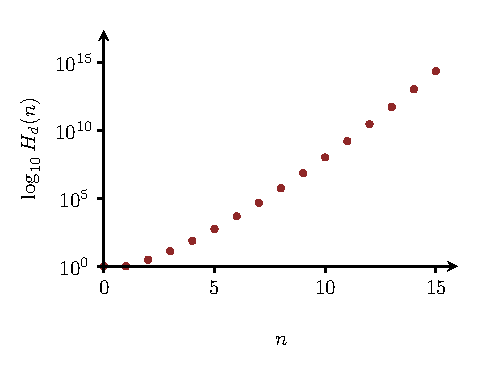
\includegraphics[width=0.75\textwidth,height=\textheight]{figures/bell/bell.pdf}

}

\caption{\label{fig-bell}The \(n\)th ordered Bell number counts the
number of ordered partitions of a finite set with \(n\) elements. As the
size of a set increases, the number of ordered partitions increases
extraordinarily quickly. Even on a log scale the growth appears to be
exponential!}

\end{figure}%

\subsection{Atomic Conditional
Decompositions}\label{atomic-conditional-decompositions}

That said, most practical applications consider only \textbf{atomic
conditional decompositions} that decompose joint probability
distributions as completely as possible.

An atomic conditional decomposition is defined by an atomic partition,
where each cell consists of only a single component index, \[
\mathsf{i}_{k} = \{ i_{k}  \}.
\] This results in the sequence of conditional probability kernels \[
\pi(
  \mathsf{x}_{ \{ \mathsf{i}_{k}  \} } \mid
  x_{\mathsf{j}_{k + 1}}
)
\] and the marginal probability distribution, \[
\pi( \mathsf{x}_{ \mathsf{j}_{I} } ).
\] These conditional decomposition ``peel'' off one component space at a
time in the prescribed order.

Given \(I\) component spaces, there are only \(I!\) of these atomic
conditional decompositions, each corresponding to a particular ordering
of the components. The number of atomic conditional decompositions grows
quickly with as the number of component spaces, but far less so than the
number of general conditional decompositions does.

For instance, when working with the product space \[
X^{1:3} = X_{1} \times X_{2} \times X_{3},
\] we have only six unique atomic conditional decompositions
corresponding to the partitions \begin{align*}
&( \; ( 1 ), ( 2 ), ( 3 ) \; ); \quad
 ( \; ( 1 ), ( 3 ), ( 2 ) \; ); \quad
 ( \; ( 2 ), ( 1 ), ( 3 ) \; );
\\
&( \; ( 2 ), ( 3 ), ( 1 ) \; ); \quad
 ( \; ( 3 ), ( 1 ), ( 2 ) \; ); \quad
 ( \; ( 3 ), ( 2 ), ( 1 ) \; ).
\end{align*}

To exhaustively demonstrate, the partition
\(( \; ( 2 ), ( 3 ), ( 1 ) \; )\) defines the atomic conditional
decomposition \[
\pi( \mathrm{d} x_{1}, \mathrm{d} x_{2}, \mathrm{d} x_{3} )
=
\pi( \mathrm{d} x_{2} \mid \mathrm{d} x_{1}, \mathrm{d} x_{3} ) \,
\pi( \mathrm{d} x_{3} \mid \mathrm{d} x_{1} ) \,
\pi( \mathrm{d} x_{1} ).
\] This is equivalent to the decomposition of the joint probability
density function into conditional and marginal probability density
functions, \[
p( x_{1}, x_{2}, x_{3} )
=
p( x_{2} \mid x_{1}, x_{3} ) \,
p( x_{3} \mid x_{1} ) \,
p( x_{1} ).
\]

\section{Sequential Construction of Joint Probability
Distributions}\label{sequential-construction-of-joint-probability-distributions}

While the names suggests destruction, conditional decompositions can
also be used to \emph{construct} joint probability distributions from
simpler probabilistic pieces.

Given a partition of the component indices, we can construct a joint
distribution by working through the subsequences of component indices
\emph{in reverse}. After engineering an appropriate marginal
distribution \[
\pi( \mathsf{x}_{ \mathsf{j}_{K} } )
\] over the thinned product space \(X^{ \mathsf{j}_{K} }\), we engineer
conditional probability kernels, \[
\pi( \mathsf{x}_{ \mathsf{i}_{k} } \mid x_{\mathsf{j}_{k + 1}} )
\] over the cross sections \[
X^{ \mathsf{i}_{k} } \times \{ x_{ \mathsf{j}_{k + 1} }   ).
\] The ultimate conditional probability kernel lifts
\(\pi( \mathsf{x}_{ \mathsf{j}_{K} } )\) into a joint distribution over
\(X^{ \mathsf{j}_{K - 1} }\), before the penultimate conditional
probability kernel lifts that joint distribution into a joint
distribution over \(X^{ \mathsf{j}_{K - 2} }\), and so on. Altogether,
the conditional probability kernels lift the marginal distribution into
a joint distribution over the full product space.

When the \(\mathsf{i}_{k}\) are small, the intermediate cross sections
will be simple compared to the full product space. In this case
engineering probabilistic objects over the cross sections will typically
be more manageable than trying to work with the entire product space at
once. For example, when building off of an atomic decomposition, we will
only ever have to work with a single active component space at a time,
starting with \[
\pi( \mathsf{x}_{ i_{I} } ),
\] and then proceeding to each \[
\pi(
  \mathsf{x}_{ i_{k} } \mid
  x_{ i_{k + 1} }, \ldots, x_{ i_{I} }.
)
\]

In other words, conditional decompositions define a kind of armature
around which we can design joint distributions. Once the structure of
armature has been established with the choice of a conditional
decomposition, we can focus on the details, namely the choice of the
marginal distribution and each conditional probability kernel.

\section{Structured Conditional
Decompositions}\label{structured-conditional-decompositions}

In many applications, the conditional probability kernels in a
conditional decomposition will behave simpler than what is strictly
possible. These simplifications, in turn, encode meaningful structure of
the corresponding joint distributions. To take advantage of this
structure in practice, however, we will need to establish an appropriate
vocabulary.

\section{Conditional Dependencies}\label{conditional-dependencies}

At any step of a conditional decomposition, the behavior of the
conditional probability distributions will, in general, depend on the
behavior of \emph{all} of the remaining component spaces, \[
\pi( \mathsf{x}_{ \mathsf{i}_{k} } \mid x_{\mathsf{j}_{k + 1}} )
\] where \[
\mathsf{j}_{k + 1}
=
\vec{\cup}_{k' = k + 1}^{K} \mathsf{i}_{k'}.
\] In this case, we say that the conditional probability kernel is
\textbf{conditionally dependent} on the behavior in each thinned product
space \[
X^{ \mathsf{i}_{k + 1} }, X^{ \mathsf{i}_{k + 2} }, \ldots,
X^{ \mathsf{i}_{K - 1} }, X^{ \mathsf{i}_{K} }.
\]

Sometimes, however, the behavior of the conditional probability
distributions at one step will be invariant to the behavior in some of
these thinned product spaces. For example, if \[
\pi(
  \mathsf{x}_{ \mathsf{i}_{k} } \mid
  x_{ \mathsf{i}_{k + 3} \vec{\cup} \mathsf{i}_{K - 1} }
),
\] then the conditional probability kernel will be conditionally
dependent on only \(X^{ \mathsf{i}_{k + 3} }\) and
\(X^{ \mathsf{i}_{K - 1} }\).

Note that we are considering dependencies on not individual component
spaces but rather the particular thinned product spaces defined by the
component index partition. If we want to allow for more precise
conditional dependencies, then we need to use a finer partition of the
component indices. In this sense, the conditional dependencies from
atomic conditional decompositions are the most informative.

Conditional dependencies also neatly translate into the structure of
conditional probability density functions. For example, if \[
\pi(
  \mathsf{x}_{ \mathsf{i}_{k} } \mid
  x_{ \mathsf{i}_{k + 3} \vec{\cup} \mathsf{i}_{K - 1} }
)
\] then we would also have \[
p(
  x_{ \mathsf{i}_{k} } \mid
  x_{ \mathsf{i}_{k + 3} \vec{\cup} \mathsf{i}_{K - 1} }
).
\]

\subsection{Conditional
Independencies}\label{conditional-independencies}

An important, but subtle, aspect of conditional dependencies is that
define only \emph{direct} or \emph{local} dependencies. For instance,
the conditional behavior of \(x_{ \mathsf{i}_{k} }\) may not
conditionally depend on the behavior of \(x_{ \mathsf{i}_{k'} }\). If,
however, \(x_{ \mathsf{i}_{k} }\) conditionally depends on
\(x_{ \mathsf{i}_{k''} }\) and \(x_{ \mathsf{i}_{k''} }\) itself
conditionally depends on \(x_{ \mathsf{i}_{k'} }\), then
\(x_{ \mathsf{i}_{k'} }\) will \emph{indirectly} moderate
\(x_{ \mathsf{i}_{k} }\) through \(x_{ \mathsf{i}_{k''} }\).

To check for these indirect dependencies we have to push the joint
probability distribution forward along the projection function \[
\varpi_{ \mathsf{i}_{k} \, \vec{\subset} \, \mathsf{i}_{k'} } :
X^{1:I}
\rightarrow
X^{ \mathsf{i}_{k} \, \vec{\subset} \, \mathsf{i}_{k'} },
\] and then disintegrate that pushforward distribution with respect to
the projection function \[
\varpi^{ \mathsf{i}_{k} \, \vec{\subset} \,
         \mathsf{i}_{k'} }_{ \mathsf{i}_{k'} } :
X^{ \mathsf{i}_{k} \, \vec{\subset} \, \mathsf{i}_{k'} }
\rightarrow
X^{ \mathsf{i}_{k'} }.
\] If the resulting conditional probability kernel is invariant to the
behavior in \(X^{ \mathsf{i}_{k'} }\), \[
\pi( \mathsf{x}_{ \mathsf{i}_{k} } \mid \mathsf{i}_{k'} )
=
\pi( \mathsf{x}_{ \mathsf{i}_{k} } ),
\] then the conditional behavior of \(x_{ \mathsf{i}_{k} }\) will be
completely independent of \(x_{ \mathsf{i}_{k'} }\), regardless of the
behavior of any other component spaces. In this case, we say that
\(x_{ \mathsf{i}_{k} }\) is \textbf{conditionally independent} of
\(x_{ \mathsf{i}_{k'} }\).

More generally, if we apply this procedure not to joint distribution \[
\pi( \mathsf{x}_{ 1:I } )
\] but rather to the conditional probability kernel \[
\pi(
  \mathsf{x}_{ \mathsf{i}_{k''}^{c} } \mid
  x_{ \mathsf{i}_{k''} }
)
\] and \[
\pi(
  \mathsf{x}_{ \mathsf{i}_{k} } \mid
  x_{ \mathsf{i}_{k'} \vec{\subset} \mathsf{i}_{k''} }
)
=
\pi( \mathsf{x}_{ \mathsf{i}_{k} } \mid x_{ \mathsf{i}_{k''} } ),
\] then we say that \(x_{ \mathsf{i}_{k} }\) is conditionally
independent of \(x_{ \mathsf{i}_{k'} }\) given
\(x_{ \mathsf{i}_{k''} }\).

While conditional dependencies are straightforward, conditional
independencies are often counter-intuitive and require careful
consideration. For much more on conditional independences for atomic
conditional decompostions, see Bishop (2006).

\subsection{Dependency Subsequences}\label{dependency-subsequences}

Conditional dependencies are not unique to any one choice of conditional
probability kernel. Indeed, different conditional probability kernels
can share the same conditional dependencies. Fortunately, abstracting
the conditional dependencies from any particular conditional probability
kernel is straightforward.

At the \(k\)th step of a conditional decomposition, any valid
conditional probability kernel can depend on the thinned product spaces
given by the subsequences of component indices \[
\mathsf{i}_{k + 1}, \mathsf{i}_{k + 2}, \ldots,
\mathsf{i}_{K - 1}, \mathsf{i}_{K}.
\] We can neatly communicate the dependencies between these subsequences
by collecting them into subsets, \[
\mathsf{d}_{k}
=
\{
  \mathsf{i}_{k'} \mid
   k' \in \mathsf{k}_{k} \subset \{ k + 1, \ldots, K \}
\}.
\] This allows us to write the conditional probability kernel more
precisely as \[
\pi( \mathsf{x}_{ \mathsf{i}_{k} } \mid \mathsf{d}_{k} ).
\] I will refer to these subsequences as \textbf{dependency
subsequences}.

For example, the last dependency subsequence is always empty because
there are no component spaces left on which behavior can depend, \[
\mathsf{d}_{K} = ().
\] The second-to-last dependency subsequence, however, could be one of
two possibilities, \[
\mathsf{d}_{K - 1} = ()
\] or \[
\mathsf{d}_{K - 1} = \mathsf{i}_{K},
\] while the third-to-last could be one of four possibilities,
\begin{align*}
\mathsf{d}_{K - 2} &= ()
\\
\mathsf{d}_{K - 2} &= \mathsf{i}_{K - 1}
\\
\mathsf{d}_{K - 2}
&=
\{ \mathsf{i}_{K - 1}, \mathsf{i}_{K} \}
\\
\mathsf{d}_{K - 2} &= \mathsf{i}_{K}.
\end{align*}

Dependency subsequences allow us to incorporate even more information
into a conditional decomposition without having to commit to particular
conditional probability kernels and marginal distributions.
Specifically, we can generalize a conditional decomposition to be a
sequence of pairs, \[
( ( \mathsf{i}_{1}, \mathsf{d}_{1}), \ldots,
  ( \mathsf{i}_{K}, \mathsf{d}_{K} ),
\] where the \(\mathsf{i}_{k}\) partition the component indices and the
\(\mathsf{d}_{k}\) communicate the precise conditional dependencies.

If, for instance, we have an atomic conditional decomposition and \[
\mathsf{d}_{k} = \emptyset
\] for all \(k\), then every conditional probability distribution will
be independent of the behavior in every subsequent component space, \[
\pi( \mathsf{x}_{ i_{k} } \mid \mathsf{d}_{k} )
=
\pi( \mathsf{x}_{ i_{k} } ).
\] In this case, the joint distribution will be an independent product
distribution, \[
\pi( \mathrm{d} x_{1}, \ldots, \mathrm{d} x_{I} )
=
\pi( \mathrm{d} x_{1} ) \,
\ldots \,
\pi( \mathrm{d} x_{i}  ) \,
\ldots \,
\pi( \mathrm{d} x_{I} ).
\] Conditional dependencies give us yet another way to characterize
independent product distributions!

For a more specific example, consider the product space \[
X = X_{1} \times X_{2} \times X_{3} \times X_{4}
\] with the atomic conditional decomposition \[
( \;
  ( \; ( 4 ), \{ (1), (3) \} \; ),  \quad
  ( \; ( 3 ), \{ (1), (2) \} \; ),  \quad
  ( \; ( 1 ), \{ (2)      \} \; ),  \quad
  ( \; ( 2 ), \emptyset      \; )
\; ).
\] Any joint probability density function compatible with this
conditional decomposition will be of the form \begin{align*}
p( x_{1}, x_{2}, x_{3}, x_{4} )
&= \;\,
p( x_{4} \mid x_{1}, x_{3} )
\\
&\quad \cdot
p( x_{3} \mid x_{1}, x_{2} )
\\
&\quad \cdot
p( x_{1} \mid x_{2} )
\\
&\quad \cdot
p( x_{2} ).
\end{align*}

With dependency subsequences, our probabilistic modeling armature
becomes even more informative. We can now construct joint distributions
in three stages: partitioning the component variables into subsequences,
specifying the precise conditional dependencies between these
subsequences, and then finally specifying particular conditional
probability kernels and a particular marginal distribution.

\section{Directed Graphical Models}\label{directed-graphical-models}

While richly informative, component index partitions and dependency
subsequences can be awkward to work with in practice. Reading off
conditional dependencies from the structure of conditional probability
densities is less explicit but often more intuitive to many
practitioners. In this section, we will consider a \emph{visual}
representation of conditional decompositions that neatly complements
these approaches.

\subsection{Directed Acyclic Graphs}\label{directed-acyclic-graphs}

A \textbf{graph} is a collection of \textbf{nodes} with \textbf{edges}
connecting certain pairs of nodes. Typically, nodes represent
mathematical objects and edges the relationships, or lack thereof,
between them.

\textbf{Directed graphs} distinguish between edges that originate from
one node and terminate in another, and vice versa. The structure of a
directed graph is particularly straightforward to visualize, with
two-dimensional shapes representing each node and one-dimensional arrows
the directed edges connecting them (Figure~\ref{fig-dgm1}).

\begin{figure}

\centering{

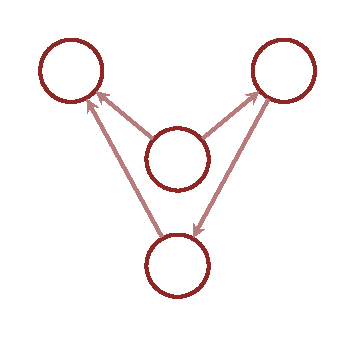
\includegraphics[width=0.33\textwidth,height=\textheight]{figures/dgms/1/dg.pdf}

}

\caption{\label{fig-dgm1}Directed graphs are typically visualized with
shapes to represent each node and arrows to represent the directed edges
between them. When the nodes of a directed graph are named, we can also
label the shapes accordingly.}

\end{figure}%

The nodes at which a directed edge originates is referred to as the
\textbf{parent} of the node at which the edge terminates. Similarly, the
terminating node is referred to as a \textbf{child} of originating node
(Figure~\ref{fig-dgm2}). This familial language motivates a variety of
related vocabulary, such as referring to two nodes that share a common
parent as siblings.

\begin{figure}

\centering{

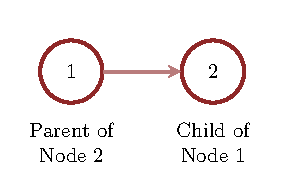
\includegraphics[width=0.33\textwidth,height=\textheight]{figures/dgms/2/dg.pdf}

}

\caption{\label{fig-dgm2}Two nodes connected by a directed edge are
referred to as the parent and child of each other. This terminology
allows us to compactly describe relationships between nodes in a
directed graph.}

\end{figure}%

A sequence of directed edges connecting parent nodes to child nodes
defines a \textbf{path} through the graph. In general, these paths can
circle back on themselves, forming \textbf{cycles}
(Figure~\ref{fig-dgm3}). Directed graphs that do not exhibit any cycles
(Figure~\ref{fig-dgm4}) are known as \textbf{directed acyclic graphs},
or just \textbf{DAGs} for short.

\begin{figure}

\begin{minipage}{0.15\linewidth}
~\end{minipage}%
%
\begin{minipage}{0.35\linewidth}

\centering{

\captionsetup{labelsep=none}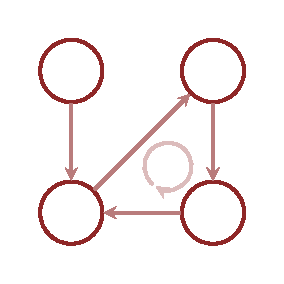
\includegraphics{figures/dgms/3/dg.pdf}

}

\subcaption{\label{fig-dgm3}}

\end{minipage}%
%
\begin{minipage}{0.35\linewidth}

\centering{

\captionsetup{labelsep=none}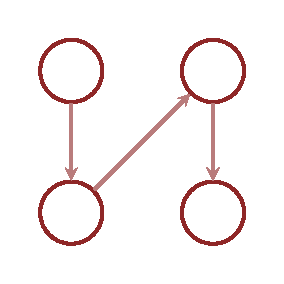
\includegraphics{figures/dgms/4/dg.pdf}

}

\subcaption{\label{fig-dgm4}}

\end{minipage}%
%
\begin{minipage}{0.15\linewidth}
~\end{minipage}%

\caption{\label{fig-dags}(a) Cycles in a directed graph are formed by
paths of directed edges that connect back on themselves. (b) In a
directed acyclic graph, each path originates and terminates at a
distinct node.}

\end{figure}%

Because of the lack of cycles, directed acyclic graphs exhibit a
well-defined notion of directionality (Figure~\ref{fig-dgm5}). On one
side of the graph we have \textbf{root nodes} with no parents, and on
the other we have \textbf{leaf nodes} with no children.

\begin{figure}

\centering{

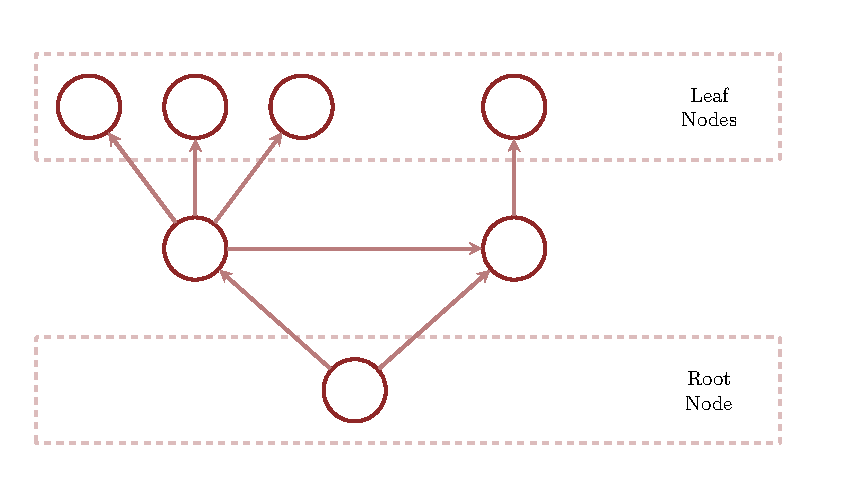
\includegraphics[width=1\textwidth,height=\textheight]{figures/dgms/5/dg.pdf}

}

\caption{\label{fig-dgm5}Directed acyclic graph can be arranged in a
natural direction, starting with root nodes that have no parents and
ending with leaf nodes that have no children.}

\end{figure}%

Although visualizations of directed graphs don't technically have to
respect this directionality, they tend to be more effective when they
do. That said, there is no universal convention for whether root notes
should be on the top, bottom, left, or right of a visualization. We are
free to pick whichever convention is most convenient, although it's best
to maintain that convention consistently.

\subsection{Graphical Models of Conditional
Decompositions}\label{graphical-models-of-conditional-decompositions}

Conveniently, every atomic conditional decomposition defines a unique
directed acyclic graph, which can then be used to visualize the
conditional structure. A conditional decomposition represented by a
directed acyclic graph is known as a \textbf{directed graphical model},
\textbf{graphical model}, or even just \textbf{DGM}.

To see how to translate a conditional decomposition into a graphical
model, let's consider the general conditional decomposition \[
( ( \mathsf{i}_{1}, \mathsf{d}_{1} ), \quad
  \ldots, \quad
  ( \mathsf{i}_{K}, \mathsf{d}_{K} ) ).
\] Each subsequence of active component indices, \[
\mathsf{i}_{k}
\] can be represented by a node labeled with the corresponding component
variables. The elements of \(\mathsf{d}_{k}\) then define arrows that
originate at the node representing the corresponding component indices
and terminating at \(\mathsf{i}_{k}\).

To demonstrate, let's take \(I = 8\) and build a graphical model for the
the conditional decomposition \begin{alignat*}{8}
(& \;\; &( \; &( 1, 7 ),& &\{ (2), (3, 4, 5) &\} \; &), &
\\
 & &( \; &(3, 4, 5),& \; &\{ (2) &\} \; &), &
\\
 & &( \;  &(2),& &\{ (6, 8) &\} \; &), &
\\
 & &( \;   &(6, 8),& &\{ &\}\; &), &\;\;)
\end{alignat*} This corresponds to the joint probability density
function decomposition \begin{align*}
p( x_{1}, &x_{2}, x_{3}, x_{4}, x_{5}, x_{6}, x_{7}, x_{8} )
\\
&= \;\,
p( x_{1}, x_{7} \mid x_{2}, x_{3}, x_{4}, x_{5} )
\\
&\quad \cdot
p( x_{3}, x_{4}, x_{5} \mid x_{2} )
\\
&\quad \cdot
p( x_{2} \mid x_{6}, x_{8} )
\\
&\quad \cdot
p( x_{6}, x_{8} ).
\end{align*}

The four component index subsequences \begin{align*}
\mathsf{i}_{1} &= ( 1, 7 )
\\
\mathsf{i}_{2} &= ( 3, 4, 5 )
\\
\mathsf{i}_{3} &= ( 2 )
\\
\mathsf{i}_{4} &= ( 6, 8 )
\end{align*} each define a node in the corresponding graphical model
(Figure~\ref{fig-dgm6a}).

Because \(x_{ \mathsf{i}_{1} }\) directly depends on both
\(x_{ \mathsf{i}_{2} }\) and \(x_{ \mathsf{i}_{3} }\), we next place two
direct edges between the corresponding nodes (Figure~\ref{fig-dgm6b}).
Similarly, we place a lone directed edge that terminates at
\(x_{ \mathsf{i}_{2} }\). (Figure~\ref{fig-dgm6c}). Finally, we place
one last directed edge from the node representing
\(x_{ \mathsf{i}_{4} }\) to the node representing
\(x_{ \mathsf{i}_{3} }\) (Figure~\ref{fig-dgm6d}). Lacking any
conditional dependencies, no directed edges terminate at
\(x_{ \mathsf{i}_{4} }\). In this case, the node representing
\(x_{ \mathsf{i}_{1} }\) defines a lone leaf node, while the node
representing \(x_{ \mathsf{i}_{4} }\) defines the only root node.

\begin{figure}

\begin{minipage}{0.10\linewidth}
~\end{minipage}%
%
\begin{minipage}{0.40\linewidth}

\centering{

\captionsetup{labelsep=none}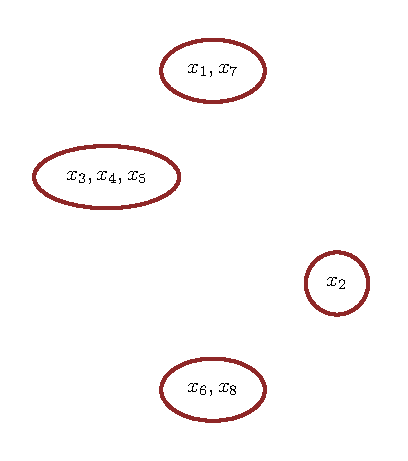
\includegraphics{figures/dgms/6a/dg.pdf}

}

\subcaption{\label{fig-dgm6a}}

\end{minipage}%
%
\begin{minipage}{0.40\linewidth}

\centering{

\captionsetup{labelsep=none}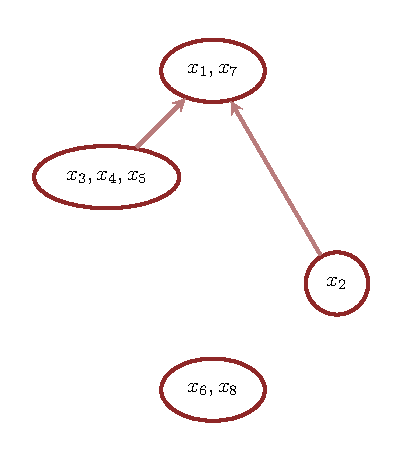
\includegraphics{figures/dgms/6b/dg.pdf}

}

\subcaption{\label{fig-dgm6b}}

\end{minipage}%
%
\begin{minipage}{0.10\linewidth}
~\end{minipage}%
\newline
\begin{minipage}{0.10\linewidth}
~\end{minipage}%
%
\begin{minipage}{0.40\linewidth}

\centering{

\captionsetup{labelsep=none}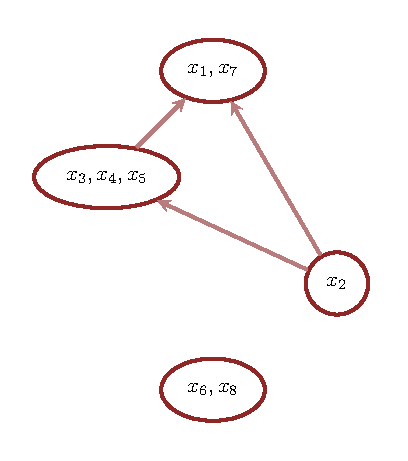
\includegraphics{figures/dgms/6c/dg.pdf}

}

\subcaption{\label{fig-dgm6c}}

\end{minipage}%
%
\begin{minipage}{0.40\linewidth}

\centering{

\captionsetup{labelsep=none}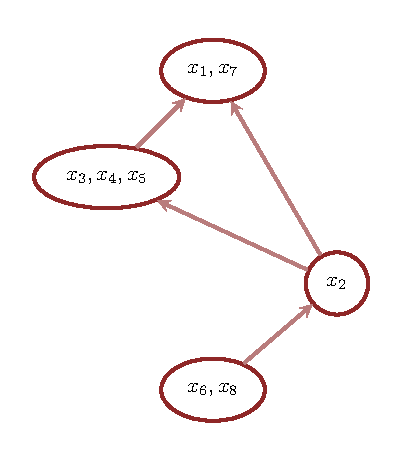
\includegraphics{figures/dgms/6d/dg.pdf}

}

\subcaption{\label{fig-dgm6d}}

\end{minipage}%
%
\begin{minipage}{0.10\linewidth}
~\end{minipage}%

\caption{\label{fig-dgm6}Graphical models are straightforward to build
for atomic conditional decompositions. (a) After placing nodes for each
subsequence of active component spaces, (b-d) we work down the
conditional decomposition, placing directed arrows nodes that are
conditionally dependent on each other.}

\end{figure}%

In order to probe more detailed conditional dependencies, we need to
start with more refined partitions of the component indices. For
example, breaking the subsequence \(\mathsf{i}_{4} = ( 6, 8 )\) up into
two subsequences \((6)\) and \((8)\) allows us to consider whether or
not \(x_{ \mathsf{i}_{3} }\) depends on \(x_{6}\), \(x_{8}\), or both.

\begin{figure}

\begin{minipage}{0.10\linewidth}
~\end{minipage}%
%
\begin{minipage}{0.40\linewidth}

\centering{

\captionsetup{labelsep=none}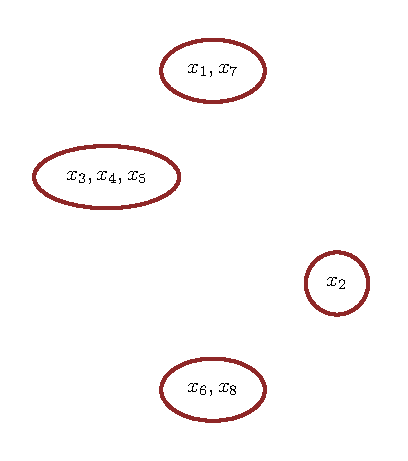
\includegraphics{figures/dgms/6a/dg.pdf}

}

\subcaption{\label{fig-dgm-refine-a}}

\end{minipage}%
%
\begin{minipage}{0.40\linewidth}

\centering{

\captionsetup{labelsep=none}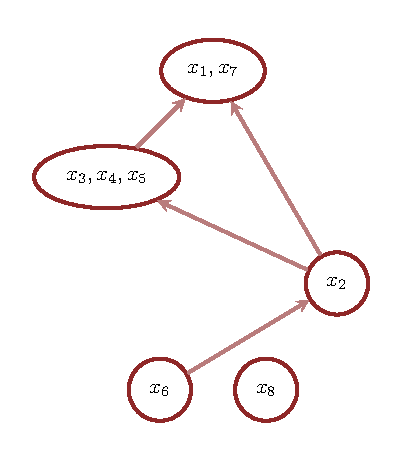
\includegraphics{figures/dgms/6e/dg.pdf}

}

\subcaption{\label{fig-dgm-refine-b}}

\end{minipage}%
%
\begin{minipage}{0.10\linewidth}
~\end{minipage}%
\newline
\begin{minipage}{0.10\linewidth}
~\end{minipage}%
%
\begin{minipage}{0.40\linewidth}

\centering{

\captionsetup{labelsep=none}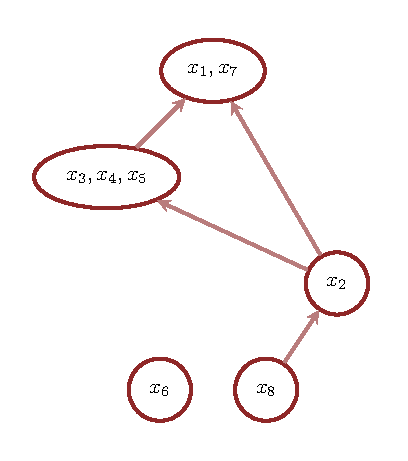
\includegraphics{figures/dgms/6f/dg.pdf}

}

\subcaption{\label{fig-dgm-refine-c}}

\end{minipage}%
%
\begin{minipage}{0.40\linewidth}

\centering{

\captionsetup{labelsep=none}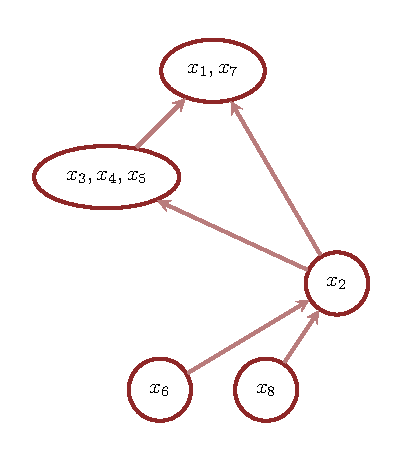
\includegraphics{figures/dgms/6g/dg.pdf}

}

\subcaption{\label{fig-dgm-refine-d}}

\end{minipage}%
%
\begin{minipage}{0.10\linewidth}
~\end{minipage}%

\caption{\label{fig-dgm-refine}(a) Directed graphical models that
visualize crude conditional decompositions can be elaborated into (b-d)
directed graphical models that visualize more more refined conditional
decompositions. In general, the many refinements will be consistent with
a given non-atomic conditional decomposition.}

\end{figure}%

That said, conditional decompositions cannot be refined beyond atomic
conditional decompositions. The corresponding directed graphical models
are a bit more straightforward, with each node representing a single
component space and each directed edge connecting pairs of component
spaces. Consider, for instance, the atomic conditional decomposition
\begin{alignat*}{8}
(& \;\; &( \; &(7),& &\{ (1), (2), (4) &\} \; &), &
\\
 & \;\; &( \; &(1),& &\{ (3), (5) &\} \; &), &
\\
 & &( \; &(4),& \; &\{  &\} \; &), &
\\
 & &( \; &(5),& \; &\{ (2), (3) &\} \; &), &
\\
 & &( \; &(3),& \; &\{ (2) &\} \; &), &
\\
 & &( \;  &(2),& &\{ (6), (8) &\} \; &), &
\\
 & &( \;   &(6),& &\{ &\}\; &), &
\\
 & &( \;   &(8),& &\{ &\}\; &) &\;\;)
\end{alignat*} This is compatible with our initial example of a
conditional decomposition, but conveys much more detailed information
about the structure of the joint probability distribution
(Figure~\ref{fig-dgm-atomic}).

\begin{figure}

\begin{minipage}{0.50\linewidth}

\centering{

\captionsetup{labelsep=none}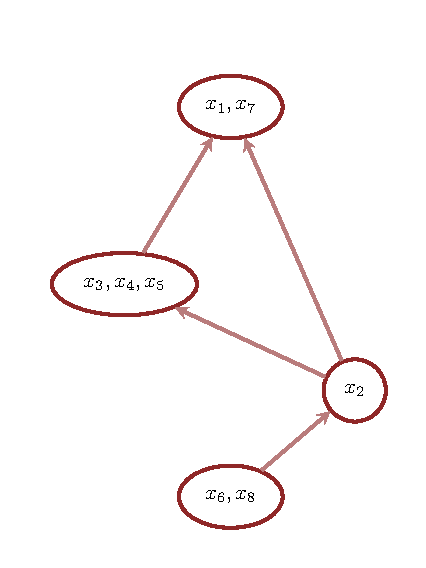
\includegraphics{figures/dgms/7a/dg.pdf}

}

\subcaption{\label{fig-dgm7a}}

\end{minipage}%
%
\begin{minipage}{0.50\linewidth}

\centering{

\captionsetup{labelsep=none}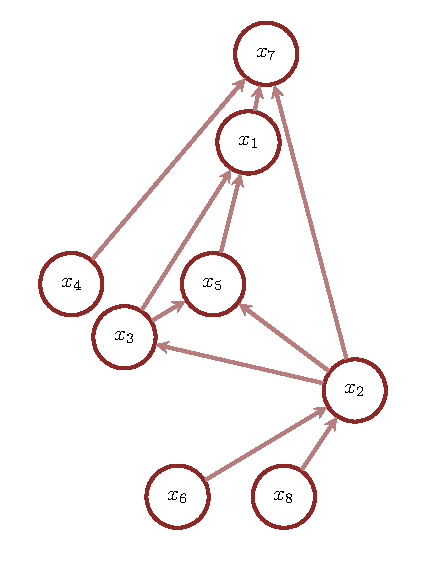
\includegraphics{figures/dgms/7b/dg.pdf}

}

\subcaption{\label{fig-dgm7b}}

\end{minipage}%

\caption{\label{fig-dgm-atomic}(a) The directed graphical models derived
from cruder compositional decompositions always contain convey less
information than (b) directed graphical models derived from atomic
conditional decompositions.}

\end{figure}%

The more coupled the behaviors in the component spaces are to each
other, the more directed edges the corresponding graphical model will
feature. Often the most informative aspect of a graphical model is the
\emph{absence} of directed edges.

\subsection{Bells and Whistles}\label{bells-and-whistles}

The nodes and edges in directed graphical models convey a wealth of
information. We can, however, pack even more information into directed
graphical models by augmenting this basic graph structure with some
special features.

\subsubsection{Auxiliary Nodes}\label{auxiliary-nodes}

Many applications consider joint distributions whose behavior depends on
the behavior of auxiliary spaces that are not equipped with any
probabilistic structure of their own. In other words, these joint
distributions are \emph{parameterized} by the configuration of the
auxiliary spaces.

These non-probabilistic dependencies can be represented in graphical
models by introducing multiple types of nodes, one to represent the
probabilistic spaces and one to represent the auxiliary spaces. I like
to use \emph{rounded} shapes to represent probabilistic nodes and
\emph{rectangular} shapes to represent auxiliary nodes.

For instance, the conditional structure of \begin{align*}
p( x_{1}, x_{2}, x_{3}, x_{4}; y )
&= \;\,
p( x_{4} \mid x_{1}, x_{3} )
\\
&\quad \cdot
p( x_{1} \mid x_{3}; y )
\\
&\quad \cdot
p( x_{3} \mid x_{2} )
\\
&\quad \cdot
p( x_{2} )
\end{align*} can be represented by the graphical model in
Figure~\ref{fig-dgm8}.

\begin{figure}

\centering{

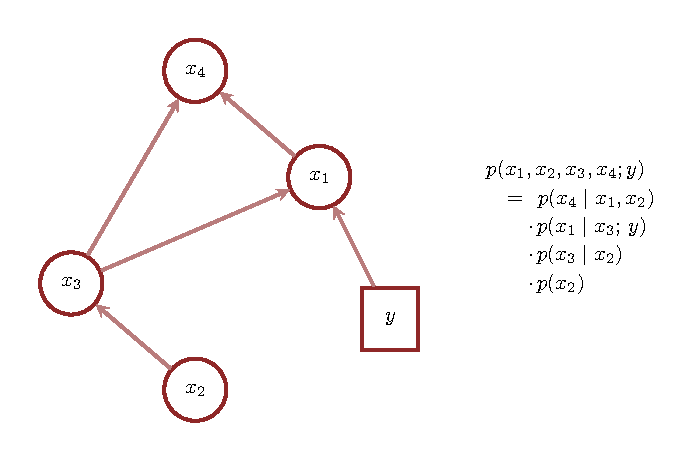
\includegraphics[width=0.75\textwidth,height=\textheight]{figures/dgms/8/dg.pdf}

}

\caption{\label{fig-dgm8}Rectangular nodes communicate non-probabilistic
dependencies in joint probability distributions. Here the conditional
density functions \(p( x_{1} \mid x_{3}; y )\) are parameterized by the
configuration of a non-probabilistic space, \(y \in Y\).}

\end{figure}%

\subsubsection{Pushforward Nodes}\label{pushforward-nodes}

Sometimes the behavior of a component space depends on the behavior of
other component spaces through only the output of some intermediate
function. For instance, instead of \begin{align*}
p( x_{1}, x_{2}, x_{3}, x_{4}; y )
&= \;\,
p( x_{4} \mid x_{1}, x_{3} )
\\
&\quad \cdot
p( x_{1} \mid x_{3}; y )
\\
&\quad \cdot
p( x_{3} \mid x_{2} )
\\
&\quad \cdot
p( x_{2} )
\end{align*} we might have \begin{align*}
p( x_{1}, x_{2}, x_{3}, x_{4}; y )
&= \;\,
p( x_{4} \mid f( x_{1}, x_{3} ) )
\\
&\quad \cdot
p( x_{1} \mid x_{3}; y )
\\
&\quad \cdot
p( x_{3} \mid x_{2} )
\\
&\quad \cdot
p( x_{2} ).
\end{align*} In this case, the behavior in \(X_{4}\) doesn't directly
depend on the behavior in \(X_{1} \times X_{3}\), but rather the
behavior in \(X_{1} \times X_{3}\) pushed forward through \(f\).

One way to communicate these functional dependencies in a graphical
model is to introduce an explicit variable for the function output,
\begin{align*}
p( x_{1}, x_{2}, x_{3}, x_{4}; y )
&= \;\,
p( x_{4} \mid y = f(x_{1}, x_{3}) )
\\
&\quad \cdot
p( x_{1} \mid x_{3}; y )
\\
&\quad \cdot
p( x_{3} \mid x_{2} )
\\
&\quad \cdot
p( x_{2} ),
\end{align*} and then represent that variable with its own node. To
avoid any ambiguity, however, we'll need to decorate this node
differently from the component nodes. I like to use dashed borders
(Figure~\ref{fig-dgm9})

\begin{figure}

\centering{

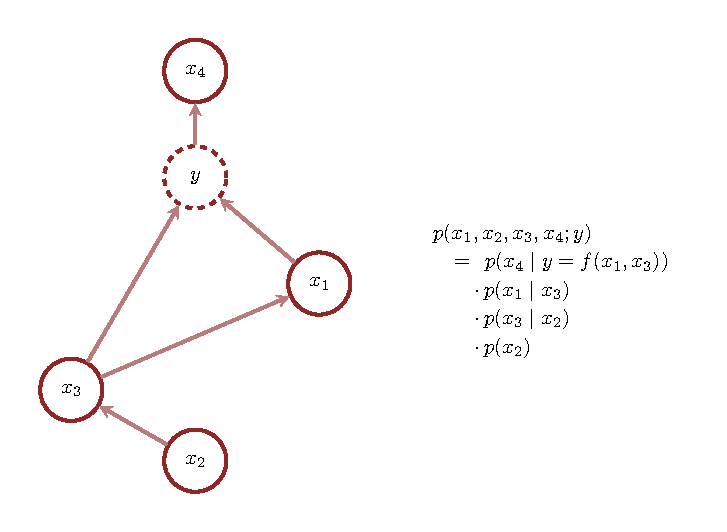
\includegraphics[width=0.75\textwidth,height=\textheight]{figures/dgms/9/dg.pdf}

}

\caption{\label{fig-dgm9}Dashed, circular nodes represent the output of
functions that depend on components variables. We can interpret these
nodes as modeling the pushforward distribution along the intermediate
function.}

\end{figure}%

\subsubsection{Conditioned Nodes}\label{conditioned-nodes}

Some applications are less concerned with a given joint distribution
than certain conditional distributions derived from that joint
distribution when we bind particular component variables to particular
values.

Once we have a graphical model for the joint distribution, this
conditioning process is straightforward to visualize by adding a
distinct decoration to the nodes corresponding to the bound variables. A
common convention is to fully color these nodes.

For example, let's say that we start with the joint distribution defined
by the probability density functions (Figure~\ref{fig-dgm10a})
\begin{align*}
p( x_{1}, x_{2}, x_{3}, x_{4} )
&= \;\,
p( x_{4} \mid x_{1}, x_{3} )
\\
&\quad \cdot
p( x_{1} \mid x_{3} )
\\&\quad \cdot
p( x_{3} \mid x_{2} )
\\
&\quad \cdot
p( x_{2} ),
\end{align*} but we are interested in the conditional distribution
defined by probability density functions \[
p( x_{2}, x_{3} \mid \tilde{x}_{1}, \tilde{x}_{4} )
=
\frac{
  p( \tilde{x}_{1}, x_{2}, x_{3}, \tilde{x}_{4} )
}{
  p( \tilde{x}_{1}, \tilde{x}_{4} ).
}
\] We can visualize this particular conditioning by coloring in the
nodes representing \(X_{1}\) and \(X_{4}\) (Figure~\ref{fig-dgm10b}).

\begin{figure}

\begin{minipage}{0.50\linewidth}

\centering{

\captionsetup{labelsep=none}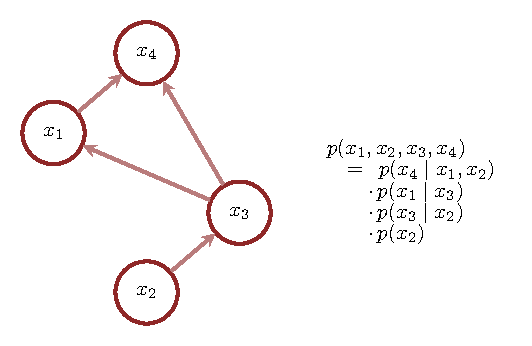
\includegraphics{figures/dgms/10a/dg.pdf}

}

\subcaption{\label{fig-dgm10a}}

\end{minipage}%
%
\begin{minipage}{0.50\linewidth}

\centering{

\captionsetup{labelsep=none}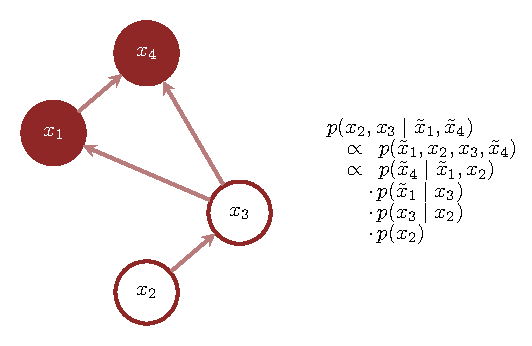
\includegraphics{figures/dgms/10b/dg.pdf}

}

\subcaption{\label{fig-dgm10b}}

\end{minipage}%

\caption{\label{fig-dgm10}The various conditional distributions that we
can derive from a joint distribution can be represented by (a) taking
the graphical model for the joint distribution and (b) coloring in the
nodes representing the components being bound to particular values.}

\end{figure}%

\subsubsection{Plate Notation}\label{plate-notation}

Some patterns of conditional dependencies are sufficiently common that
it's useful to introduce graphical shorthands that allow for more
compact visualizations.

Consider, for example, the product space \(X = X^{1:5}\), and the
conditional decomposition \begin{alignat*}{8}
(& \;\; &( \; &(1),& &\{ (5) &\} \; &), &
\\
 & \;\; &( \; &(2),& &\{ (5) &\} \; &), &
\\
 & &( \; &(3),& \; &\{ (5) &\} \; &), &
\\
 & &( \; &(4),& \; &\{ (5) &\} \; &), &
\\
 & &( \; &(5),& \; &\{ (5) &\} \; &)  &\;\;)
\end{alignat*} or, equivalently, the sequence of probability density
functions \begin{align*}
p( x_{1}, x_{2}, x_{3}, x_{4}, x_{5} )
&= \;\,
p( x_{1} \mid x_{5} )
\\
&\quad \cdot
p( x_{2} \mid x_{5} )
\\
&\quad \cdot
p( x_{3} \mid x_{5} )
\\
&\quad \cdot
p( x_{4} \mid x_{5} )
\\
&\quad \cdot
p( x_{5} ).
\end{align*}

This particular conditional structure results in a fan-like graphical
model (Figure~\ref{fig-dgm11}), which can take up a lot of visual space.
We can make the graphical model a bit more compact, however, by packing
the first four nodes together into a single \textbf{plate} that
represents their common dependence on the fifth node.

\begin{figure}

\begin{minipage}{0.50\linewidth}

\centering{

\captionsetup{labelsep=none}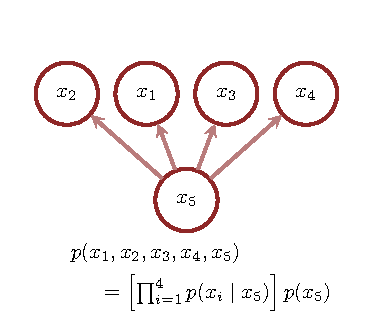
\includegraphics{figures/dgms/11/dg.pdf}

}

\subcaption{\label{fig-dgm11}}

\end{minipage}%
%
\begin{minipage}{0.50\linewidth}

\centering{

\captionsetup{labelsep=none}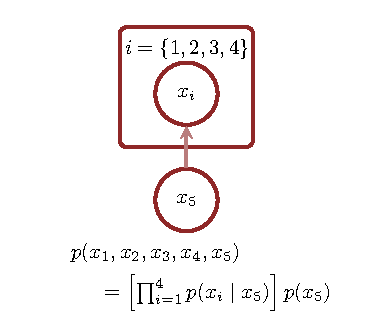
\includegraphics{figures/dgms/12/dg.pdf}

}

\subcaption{\label{fig-dgm12}}

\end{minipage}%

\caption{\label{fig-comp}(a) Conditional dependencies where many
subsequences of active components depend on one, and only one, other
subsequence of components, result in fan-like graphical models. (b)
These graphical models can be visually compressed by packing the
dependent nodes into a single plate.}

\end{figure}%

This plate notation is especially useful when we have an arbitrary
number of component spaces whose behavior conditionally depends on the
same component spaces. For instance, we might have the product space
\(X = X^{1:I} \times X_{I + 1}\) and a joint distribution built up from
the conditional decomposition \[
p( x_{1}, \ldots, x_{I + 1} )
=
\left[
  \prod_{i =  1}^{I} p( x_{i} \mid x_{I + 1} )
\right] \,
p ( x_{I + 1} ).
\]

We can try to construct heuristic visualizations to represent the
arbitrary number of nodes (Figure~\ref{fig-dgm13}), but the plate
notation allow us to visualize this structure exactly
(Figure~\ref{fig-dgm14}).

\begin{figure}

\begin{minipage}{0.50\linewidth}

\centering{

\captionsetup{labelsep=none}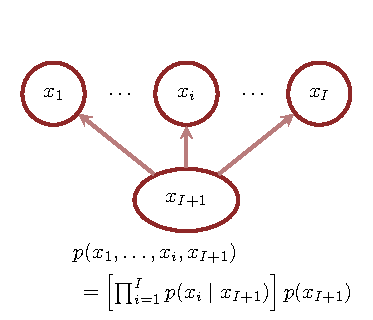
\includegraphics{figures/dgms/13/dg.pdf}

}

\subcaption{\label{fig-dgm13}}

\end{minipage}%
%
\begin{minipage}{0.50\linewidth}

\centering{

\captionsetup{labelsep=none}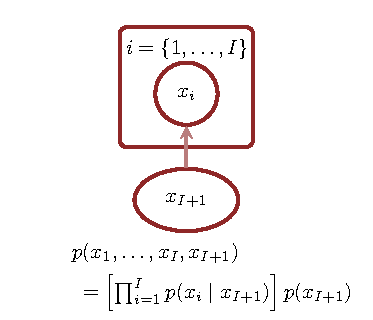
\includegraphics{figures/dgms/14/dg.pdf}

}

\subcaption{\label{fig-dgm14}}

\end{minipage}%

\caption{\label{fig-comp}(a) Graphical models with an arbitrary number
of nodes are awkward to visualize. (b) When applicable, plates avoid
this awkwardness entirely.}

\end{figure}%

Plates can also be nested to accommodate \emph{hierarchical conditional
dependencies}

\begin{figure}

\begin{minipage}{0.15\linewidth}
~\end{minipage}%
%
\begin{minipage}{0.70\linewidth}

\centering{

\captionsetup{labelsep=none}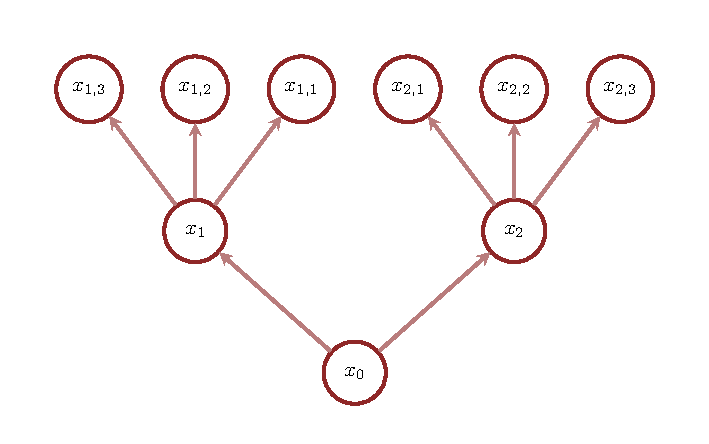
\includegraphics{figures/dgms/15/dg.pdf}

}

\subcaption{\label{fig-dgm15}}

\end{minipage}%
%
\begin{minipage}{0.15\linewidth}
~\end{minipage}%
\newline
\begin{minipage}{0.15\linewidth}
~\end{minipage}%
%
\begin{minipage}{0.70\linewidth}

\centering{

\captionsetup{labelsep=none}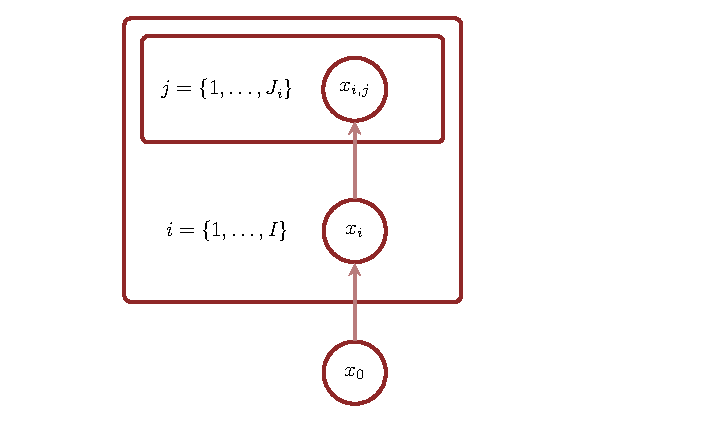
\includegraphics{figures/dgms/16/dg.pdf}

}

\subcaption{\label{fig-dgm16}}

\end{minipage}%
%
\begin{minipage}{0.15\linewidth}
~\end{minipage}%

\caption{\label{fig-comp}(a) Nested hierarchies of conditional
dependencies can also be compactly visualized by (b) nested plates
within other plates.}

\end{figure}%

\subsection{Subtleties and
Limitations}\label{subtleties-and-limitations}

Directed graphical models can be a powerful tool for communicating the
structure of conditional decompositions in practice, especially as a
complement to explicit probability density functions. That said,
directed graphical models are not without subtleties and limitations
that require some care.

For instance, directed graphical models communicate the structure of a
particular \emph{conditional decomposition}, not a particular
\emph{joint distribution}. The same joint distribution under different
partitions of the component indices will result in different graphical
models. At the same time, different joint distributions with the same
conditional dependencies will correspond to the same graphical model,
just with differences in the particular conditional distributions and/or
marginal distribution.

In other words, joint distributions alone do not define unique graphical
models, and graphical models alone do not completely define joint
distributions. In order to communicate the details of a particular joint
distribution, we need to complement a graphical model with additional
information.

Another potential issue is that transforming a joint distribution will,
in general, transform the corresponding graphical model. Transformations
that preserve the product structure of a space will, by definition, also
preserve the structure of conditional decompositions, and hence the
structure of graphical models. For instance, we can freely transform
individual component spaces without affecting the graphical modeling
representation. On the other hand, transformations that reorder the
component spaces or mix them together will change conditional
decompositions, and hence the corresponding graphical models.

One of the more frustrating aspects of directed graphical models is that
they can struggle to effectively communicate certain operations.
Consider, for example, the joint distribution defined by the density
function decomposition \begin{align*}
p( x_{1}, \ldots, x_{6}  )
&= \;\,
p ( x_{1} \mid x_{4} - x_{6} )
\\&\quad \cdot
p ( x_{2} \mid x_{6} - x_{5} )
\\
&\quad \cdot
p ( x_{3} \mid x_{5} - x_{4} )
\\
&\quad \cdot
p ( x_{4} ) \,
p ( x_{5} ) \,
p ( x_{6} ).
\end{align*}

A graphical model using only six nodes, one for each \(X_{i}\), can be
confused with a more general conditional dependencies
(Figure~\ref{fig-dgm17}), \begin{align*}
p( x_{1}, \ldots, x_{6}  )
&= \;\,
p ( x_{1} \mid x_{4}, x_{6} )
\\&\quad \cdot
p ( x_{2} \mid x_{5},  x_{6} )
\\
&\quad \cdot
p ( x_{3} \mid x_{4}, x_{5} )
\\
&\quad \cdot
p ( x_{4} ) \,
p ( x_{5} ) \,
p ( x_{6} ).
\end{align*}

We can capture the conditional dependence on the differences with
pushforward nodes (Figure~\ref{fig-dgm17}), but the overlapping arrows
can be difficult to parse. Moreover, the parsing becomes only more
difficult as we add more nodes that also depend on differences between
\(x_{4}\), \(x_{5}\), and \(x_{6}\).

Another possibility is to employ plate notation
(Figure~\ref{fig-dgm19}). The problem with this approach, however, is
that each \(y_{i}\) doesn't depend on \(x_{4}\), \(x_{5}\), and
\(x_{6}\) all at the same time. Consequently, this plate diagram is
ambiguous as well.

\begin{figure}

\begin{minipage}{0.01\linewidth}
~\end{minipage}%
%
\begin{minipage}{0.33\linewidth}

\centering{

\captionsetup{labelsep=none}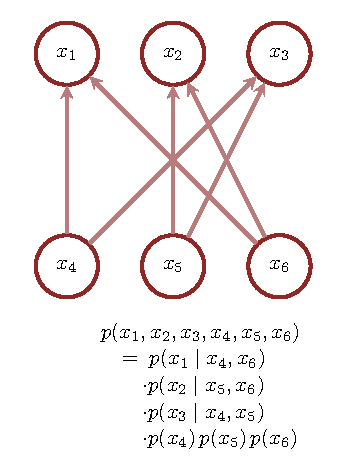
\includegraphics{figures/dgms/17/dg.pdf}

}

\subcaption{\label{fig-dgm17}}

\end{minipage}%
%
\begin{minipage}{0.33\linewidth}

\centering{

\captionsetup{labelsep=none}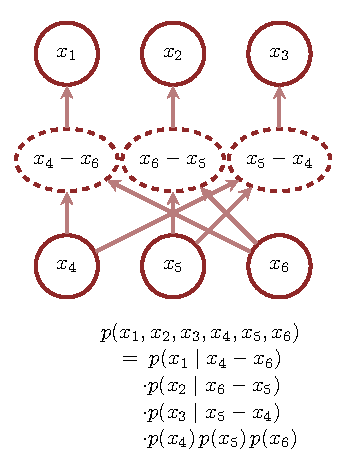
\includegraphics{figures/dgms/18/dg.pdf}

}

\subcaption{\label{fig-dgm18}}

\end{minipage}%
%
\begin{minipage}{0.33\linewidth}

\centering{

\captionsetup{labelsep=none}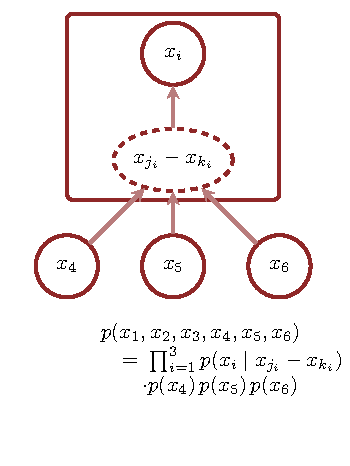
\includegraphics{figures/dgms/19/dg.pdf}

}

\subcaption{\label{fig-dgm19}}

\end{minipage}%
%
\begin{minipage}{0.01\linewidth}
~\end{minipage}%

\caption{\label{fig-comp}Some conditional structures are just awkward to
to represent with graphical models. Consider, for example, a joint
density function built up from the conditional density functions
\(p( x_{1} \mid x_{4} - x_{6} )\), \(p( x_{2} \mid x_{6} - x_{5} )\),
and \(p( x_{3} \mid x_{5} - x_{4} )\). (a) The immediate graphical model
doesn't communicate the particular dependence on the differences. (b)
Introducing pushforward nodes helps, but at the expense of a much busier
graphical model. (c) Using plates results in a more elegant graphical
model, but requires introducing conditional indices \(j_{i}\) and
\(k_{i}\) whose behavior is left ambiguous.}

\end{figure}%

All of this is to say that graphical models are not always the best tool
for communicating conditional dependencies. Sometimes a probability
density function decomposition is just more effective. Other times we
might need to reach for other representations, such as
\emph{probabilistic programming}. This will be a topic for a future
chapter.

\section{Conclusion}\label{conclusion}

Directed graphical models are a powerful tool for not only communicating
the properties of joint distributions, but also developing appropriate
joint distributions in the first place. Specifically, they allow us to
outline the basic structure of a joint distribution from the perspective
of a given partition of the component spaces, without having to consider
particular probability density functions at all. We will make extensive
use of directed graphical models once we move on to probabilistic
modeling.

\section*{Acknowledgements}\label{acknowledgements}
\addcontentsline{toc}{section}{Acknowledgements}

I thank jd for helpful comments.

A very special thanks to everyone supporting me on Patreon: Alessandro
Varacca, Alex D, Alexander Noll, Amit, Andrea Serafino, Andrew Mascioli,
Andrew Rouillard, Andrés Castro Araújo, Ara Winter, Ari Holtzman, Austin
Rochford, Aviv Keshet, Avraham Adler, Ben Matthews, Ben Swallow, Benoit
Essiambre, boot, Brendan Galdo, Bryan Chang, Cameron Smith, Canaan
Breiss, Cat Shark, Cathy Oliveri, Charles Naylor, Chase Dwelle, Chris
Jones, Christina Van Heer, Christopher Mehrvarzi, Colin Carroll, Colin
McAuliffe, Damien Mannion, dan mackinlay, Dan W Joyce, Dan Waxman, Dan
Weitzenfeld, Daniel Hammarström, Danny Van Nest, David Burdelski,
Dr.~Jobo, Dr.~Omri Har Shemesh, Dylan Maher, Dylan Spielman, Ebriand, Ed
Cashin, Eric LaMotte, Erik Banek, Eugene O'Friel, Felipe González,
Felipe Vaca, Fergus Chadwick, Francesco Corona, Geoff Rollins, Glenn
Williams, Granville Matheson, Guilherme Marthe, Hamed Bastan-Hagh,
haubur, Hector Munoz, Horace Guy, hs, Hugo Botha, Håkan Johansson, Ian
Costley, idontgetoutmuch, Ignacio Vera, Ilaria Prosdocimi, iris
pisscauldron, Isaac Vock, jacob pine, Jair Andrade, James C, James
Hodgson, James Wade, Janek Berger, Jarrett Byrnes, Jason Pekos, Jason
Wong, jd, Jeff Burnett, Jeff Dotson, Jeff Helzner, Jeffrey Erlich, Jerry
Lin , Jesper Fischer Ehmsen, Jessica Graves, Joe Sloan, John Flournoy,
Jonathan H. Morgan, Jonathon Vallejo, Josh Knecht, JU, Julian Lee,
Justin Bois, Karim Naguib, Karim Osman, Karsten Skogsholm, Konstantin
Shakhbazov, Kristian Gårdhus Wichmann, Kádár András, Lars Barquist,
lizzie , LOU ODETTE, Mads Christian Hansen, Marek Kwiatkowski, Mark
Donoghoe, Markus P., Daniel Edward Marthaler, Matthieu LEROY, Mattia
Arsendi, Matěj, Maurits van der Meer, Max, Michael Colaresi, Michael
DeJesus, Michael DeWitt, Michael Dillon, Michael Lerner, Mick Cooney,
MisterMentat , Márton Vaitkus, N Sanders, Nathaniel Burbank, Nicholas
Cowie, Nick S, Octavio Medina, Ole Rogeberg, Olivier Ma, Paolo, Pat LS,
Patrick Kelley, Patrick Boehnke, Pau Pereira Batlle, Pieter van den Berg
, ptr, quasar, Ramiro Barrantes Reynolds, Raúl Peralta Lozada, Rex,
Riccardo Fusaroli, Richard Nerland, Rob Davies, Robert Frost, Robert
Goldman, Robert kohn, Robin Taylor, Ryan Gan, Ryan Grossman, Ryan Kelly,
S Hong, Sean Wilson, Sergiy Protsiv, Seth Axen, shira, Simon Duane,
Simon Lilburn, Simon Steiger, Simone, Spencer, sssz, Stefan Lorenz,
Stephen Lienhard, Steve Forrest, Steve Harris, Steven Forrest, Stew
Watts, Stone Chen, Stoyan Georgiev, Susan Holmes, Svilup, Tate Tunstall,
Tatsuo Okubo, Teresa Ortiz, Theodore Dasher, Thomas Siegert, Thomas
Vladeck, Tobychev , Tomas Capretto, Tony Wuersch, Virgile Andreani,
Virginia Fisher, Vitalie Spinu, Vladimir M, VO2 Maximus Decius, Will
Farr, Will Lowe, Will Wen, William A Vauter, yolhaj, yureq, and Zach A.

\section*{References}\label{references}
\addcontentsline{toc}{section}{References}

\phantomsection\label{refs}
\begin{CSLReferences}{1}{0}
\bibitem[\citeproctext]{ref-Bishop:2006}
Bishop, Christopher M. 2006. \emph{Pattern Recognition and Machine
Learning}. Information Science and Statistics. Springer, New York.

\bibitem[\citeproctext]{ref-KnopfmacherEtAl:2005}
Knopfmacher, A, and M. E. Mayes. 2005. {``A Survey of Factorization
Counting Functions.''} \emph{International Journal of Number Theory} 01
(04): 563--81.

\end{CSLReferences}

\section*{License}\label{license}
\addcontentsline{toc}{section}{License}

The text and figures in this chapter are copyrighted by Michael
Betancourt and licensed under the
\href{https://creativecommons.org/licenses/by-nc/4.0/}{CC BY-NC 4.0
license}.



\end{document}
